\documentclass[conference]{IEEEtran}
\IEEEoverridecommandlockouts
% The preceding line is only needed to identify funding in the first footnote. If that is unneeded, please comment it out.
\usepackage{cite}
\usepackage{amsmath,amssymb,amsfonts}
\usepackage{algorithmic}
\usepackage{graphicx}
\usepackage{textcomp}
\usepackage{xcolor}

\RequirePackage[T1]{fontenc} 
\RequirePackage{mathptmx}    
\RequirePackage{subcaption}   
\RequirePackage{listings}   
\RequirePackage{xcolor} 
\usepackage[colorlinks,linkcolor=black,anchorcolor=black,citecolor=black]{hyperref}
\usepackage{caption}
\captionsetup{font={footnotesize}}   
\def\BibTeX{{\rm B\kern-.05em{\sc i\kern-.025em b}\kern-.08em
    T\kern-.1667em\lower.7ex\hbox{E}\kern-.125emX}}

\lstset{numbers=none,
	basicstyle=\small\ttfamily,
	numberstyle=\tiny,
	keywordstyle=\color{black}\bfseries,
	commentstyle=\color{gray},
	frame=single,
	captionpos=b, 
	rulesepcolor=\color{red!20!green!20!blue!20},
	escapeinside=``,
	xleftmargin=2em,
	xrightmargin=2em, 
	aboveskip=1em}
\begin{document}
\captionsetup{labelformat=default,labelsep=space} 

\title{\vspace*{2ex} {\Large \bfseries Paper Title (use style: \textit{paper title})} \\{\large Subtitle as needed}}

\author{
	
\IEEEauthorblockN{Authors Name/s per 1st Affiliation \textit{(Author)}}
\IEEEauthorblockA{line 1 (of \textit{Affiliation}): dept. name of organization \\
line 2: name of organization, acronyms acceptable\\
line 3: City, Country \\
\href{mailto:name@xyz.com}{\color{black}line 4: e-mail: name@xyz.com}}

\and

\IEEEauthorblockN{Authors Name/s per 2nd Affiliation \textit{(Author)}}
\IEEEauthorblockA{line 1 (of \textit{Affiliation}): dept. name of organization  \\
line 2: name of organization, acronyms acceptable \\
line 3: City, Country \\
\href{mailto:name@xyz.com}{\color{black}line 4: e-mail: name@xyz.com}}

}

\maketitle

\begin{abstract}
This electronic document is a "live" template. The various components of your paper [title, text, heads, etc.] are already defined on the style sheet, as illustrated by the portions given in this document. DO NOT USE SPECIAL CHARACTERS, SYMBOLS, OR MATH IN YOUR TITLE OR ABSTRACT.\\
\end{abstract}

\begin{IEEEkeywords}
\textit{component; formatting; style; styling; insert (keywords)}
\end{IEEEkeywords}

\section{Introduction(Heading 1)} 
All manuscripts must be in English. These guidelines include complete descriptions of the fonts, spacing, and related information for producing your proceedings manuscripts. Please follow them and if you have any questions, direct them to the production editor in charge of your proceedings at Conference Publishing Services (CPS): Phone +1 (714) 821-8380 or Fax +1 (714) 761-1784.

This template provides authors with most of the formatting specifications needed for preparing electronic versions of their papers. All standard paper components have been specified for three reasons: (1) ease of use when formatting individual papers, (2) automatic compliance to electronic requirements that facilitate the concurrent or later production of electronic products, and (3) conformity of style throughout a conference proceedings. Margins, column widths, line spacing, and type styles are built-in; examples of the type styles are provided throughout this document and are identified in italic type, within parentheses, following the example. PLEASE DO NOT RE-ADJUST THESE MARGINS. Some components, such as multi-leveled equations, graphics, and tables are not prescribed, although the various table text styles are provided. The formatter will need to create these components, incorporating the applicable criteria that follow.

\section{Type Style and Fonts} 

Wherever Times is specified, Times Roman or Times New Roman may be used. If neither is available on your word processor, please use the font closest in appearance to Times. Avoid using bit-mapped fonts if possible. True-Type 1 or Open Type fonts are preferred. Please embed symbol fonts, as well, for math, etc.

\section{Ease of Use} 

\subsection{Selecting a Template (Heading 2)} 
First, confirm that you have the correct template for your paper size. This template has been tailored for output on the US-letter paper size. If you are using A4-sized paper, please close this template and download the file for A4 paper format called "CPS\_A4\_format".

\subsection{Maintaining the Integrity of the Specifications} 
The template is used to format your paper and style the text. All margins, column widths, line spaces, and text fonts are prescribed; please do not alter them. You may note peculiarities. For example, the head margin in this template measures proportionately more than is customary. This measurement and others are deliberate, using specifications that anticipate your paper as one part of the entire proceedings, and not as an independent document. Please do not revise any of the current designations.

\section{Prepare Your Paper Before Styling} 
Before you begin to format your paper, first write and save the content as a separate text file. Keep your text and graphic files separate until after the text has been formatted and styled. Do not use hard tabs, and limit use of hard returns to only one return at the end of a paragraph. Do not add any kind of pagination anywhere in the paper. Do not number text heads-the template will do that for you.

Finally, complete content and organizational editing before formatting. Please take note of the following items when proofreading spelling and grammar:

\subsection{Abbreviations and Acronyms} 
Define abbreviations and acronyms the first time they are used in the text, even after they have been defined in the abstract. Abbreviations such as ASME, SI, MKS, CGS, sc, dc, and rms do not have to be defined. Do not use abbreviations in the title or heads unless they are unavoidable.

\subsection{Units} 

\begin{itemize}
	\item Use either SI (MKS) or CGS as primary units. (SI units are encouraged.) English units may be used as secondary units (in parentheses). An exception would be the use of English units as identifiers in trade, such as "3.5-inch disk drive". 
	
	\item Avoid combining SI and CGS units, such as current in amperes and magnetic field in oersteds. This often leads to confusion because equations do not balance dimensionally. If you must use mixed units, clearly state the units for each quantity that you use in an equation.
	
	\item Do not mix complete spellings and abbreviations of units: "Wb/m2" or "webers per square meter", not "webers/m2".  Spell out units when they appear in text: ". . . a few henries", not ". . . a few H".
	
	\item Use a zero before decimal points: "0.25", not ".25".
\end{itemize}

\subsection{Equations} 
The equations are an exception to the prescribed specifications of this template. You will need to determine whether or not your equation should be typed using either the Times New Roman or the Symbol font (please no other font). To create multileveled equations, it may be necessary to treat the equation as a graphic and insert it into the text after your paper is styled.
Number equations consecutively. Equation numbers, within parentheses, are to position flush right, as in (\ref{eq:math}), using a right tab stop. To make your equations more compact, you may use the solidus ( / ), the exp function, or appropriate exponents. Italicize Roman symbols for quantities and variables, but not Greek symbols. Use a long dash rather than a hyphen for a minus sign. Punctuate equations with commas or periods when they are part of a sentence, as in

\begin{equation}\label{eq:math}
\alpha + \beta = \chi
\end{equation}

Note that the equation is centered using a center tab stop. Be sure that the symbols in your equation have been defined before or immediately following the equation. Use "(\ref{eq:math})", not "Eq. (\ref{eq:math})" or "equation (\ref{eq:math})", except at the beginning of a sentence: "Equation (\ref{eq:math}) is . . ."

\subsection{Some Common Mistakes} 

\begin{itemize}
	\item The word "data" is plural, not singular. 
	
	\item The subscript for the permeability of vacuum 0, and other common scientific constants, is zero with subscript formatting, not a lowercase letter "o".
	
	\item In American English, commas, semi-/colons, periods, question and exclamation marks are located within quotation marks only when a complete thought or name is cited, such as a title or full quotation. When quotation marks are used, instead of a bold or italic typeface, to highlight a word or phrase, punctuation should appear outside of the quotation marks. A parenthetical phrase or statement at the end of a sentence is punctuated outside of the closing parenthesis (like this). (A parenthetical sentence is punctuated within the parentheses.)
	
	\item A graph within a graph is an "inset", not an "insert". The word alternatively is preferred to the word "alternately" (unless you really mean something that alternates).
	
	\item Do not use the word "essentially" to mean "approximately" or "effectively".
	
	\item In your paper title, if the words "that uses" can accurately replace the word "using", capitalize the "u"; if not, keep using lower-cased.
	
	\item Be aware of the different meanings of the homophones "affect" and "effect", "complement" and "compliment", "discreet" and "discrete", "principal" and "principle".
	
	\item Do not confuse "imply" and "infer".
	
	\item The prefix "non" is not a word; it should be joined to the word it modifies, usually without a hyphen.
	
	\item There is no period after the "et" in the Latin abbreviation "et al.".
	
	\item The abbreviation "i.e." means "that is", and the abbreviation "e.g." means "for example".
	
\end{itemize} 

An excellent style manual for science writers is \cite{b7}.

\section{Using the Template} 
After the text edit has been completed, the paper is ready for the template. Duplicate the template file by using the Save As command, and use the naming convention prescribed by your conference for the name of your paper. In this newly created file, highlight all of the contents and import your prepared text file. You are now ready to style your paper. 

\subsection{Authors and Affiliations} 
The template is designed so that author affiliations are not repeated each time for multiple authors of the same affiliation. Please keep your affiliations as succinct as possible (for example, do not differentiate among departments of the same organization). This template was designed for two affiliations.

\subsubsection{For author/s of only one affiliation (Heading 3)} To change the default, adjust the template as follows.

\paragraph{Selection (Heading 4)} 
Highlight all author and affiliation lines.

\paragraph{Change number of columns} 
Select Format > Columns >Presets > One Column. 

\paragraph{Deletion} 
Delete the author and affiliation lines for the second affiliation.

\paragraph{For author/s of more than two affiliations} 
To change the default, adjust the template as follows.

\paragraph{Selection} 
Highlight all author and affiliation lines.

\paragraph{Change number of columns} 
Select Format > Columns > Presets > One Column. 

\paragraph{Highlight} 
Highlight author and affiliation lines of affiliation 1 and copy this selection.

\paragraph{Formatting} 
Insert one hard return immediately after the last character of the last affiliation line. Then paste the copy of affiliation 1. Repeat as necessary for each additional affiliation.

\paragraph{Reassign number of columns} 
Place your cursor to the right of the last character of the last affiliation line of an even numbered affiliation (e.g., if there are five affiliations, place your cursor at end of fourth affiliation). Drag the cursor up to highlight all of the above author and affiliation lines. Go to Format >  Columns and select "2 Columns". If you have an odd number of affiliations, the final affiliation will be centered on the page; all previous will be in two columns.

\subsection{Identify the Headings} 
Headings, or heads, are organizational devices that guide the reader through your paper. There are two types: component heads and text heads.

Component heads identify the different components of your paper and are not topically subordinate to each other. Examples include Acknowledgments and References and, for these, the correct style to use is "Heading 5". Use "figure caption" for your Figure captions, and "table head" for your table title. Run-in heads, such as "Abstract", will require you to apply a style (in this case, italic) in addition to the style provided by the drop down menu to differentiate the head from the text.

Text heads organize the topics on a relational, hierarchical basis. For example, the paper title is the primary text head because all subsequent material relates and elaborates on this one topic. If there are two or more sub-topics, the next level head (uppercase Roman numerals) should be used and, conversely, if there are not at least two sub-topics, then no subheads should be introduced. Styles named "Heading 1", "Heading 2", "Heading 3", and "Heading 4" are prescribed.

\subsection{Figures and Tables} 

\subsubsection{Positioning Figures and Tables} 
Place figures and tables at the top and bottom of columns. Avoid placing them in the middle of columns. Large figures and tables may span across both columns. Figure captions should be below the figures; table heads should appear above the tables. Insert figures and tables (see TABLE~\ref{tab:table}) after they are cited in the text. Use the abbreviation "Fig. \ref{fig:code}", even at the beginning of a sentence.

\begin{table}[htbp]
	\caption{Table Type Styles}
	\centering \def\arraystretch{1.5}  
	\begin{center}
		\begin{tabular}{|c|c|c|c|}
			\hline
			\textbf{Table}&\multicolumn{3}{|c|}{\textbf{Table Column Head}} \\
			\cline{2-4} 
			\textbf{Head} & \textbf{\textit{Table column subhead}}& \textbf{\textit{Subhead}}& \textbf{\textit{Subhead}} \\
			\hline
			copy& More table copy$^{\mathrm{a}}$& &  \\
			\hline
			\multicolumn{4}{r}{$^{\mathrm{a}}$Sample of a Table footnote.}
		\end{tabular}
		\label{tab:table}
	\end{center}
\end{table}

\begin{figure}[htb]
	\centering
	\begin{lstlisting}[language={XML}] 
    We suggest that you use a text box 
to insert a graphic (ideally 300 dpi), 
with all fonts embedded) because, in an 
MSW document, this method is somewhat 
more stable than directly inserting a 
picture.
    To have non-visible rules on your 
frame, use the MSWord pull-down menu, 
select Format > Borders and Shading > 
Select "None".	
	\end{lstlisting} 
	\caption{Example of a ONE-COLUMN figure caption.}
	\label{fig:code}
\end{figure}

Please see last page of this document for AN EXAMPLE of a 2-COLUMN Figure (see Fig.~\ref{fig:subfig}).

Figure Labels: Use 8 point Times New Roman for Figure labels. Use words rather than symbols or abbreviations when writing Figure axis labels to avoid confusing the reader. As an example, write the quantity "Magnetization", or "Magnetization, M", not just "M". If including units in the label, present them within parentheses. Do not label axes only with units. In the example, write "Magnetization (A/m)" or "Magnetization \{A[m(1)]\}", not just "A/m". Do not label axes with a ratio of quantities and units. For example, write "Temperature (K)", not "Temperature/K".

\subsection{Footnotes} 
Use footnotes sparingly (or not at all) and place them at the bottom of the column on the page on which they are referenced. Use Times 8-point type, single-spaced. To help your readers, avoid using footnotes altogether and include necessary peripheral observations in the text (within parentheses, if you prefer, as in this sentence).

\section{Copyright Forms and Reprint Orders} 
You must submit the ASME Electronic Copyright Form (ECF) per Step 7 of the CPS author kit’s web page. THIS FORM MUST BE SUBMITTED IN ORDER TO PUBLISH YOUR PAPER.
Please see Step 9 for ordering reprints of your paper. Reprints may be ordered using the form provided as <reprint.doc> or <reprint.pdf>.

\section*{Acknowledgment}
The preferred spelling of the word "acknowledgment" in America is without an "e" after the "g". Avoid the stilted expression, "One of us (R.B.G.) thanks . . ."  Instead, try 
"R.B.G. thanks". Put applicable sponsor acknowledgments here; DO NOT place them on the first page of your paper or as a footnote.

\begin{figure*}[htb]
	\centering
	\begin{subfigure}[b]{.4\textwidth}
		\centering
		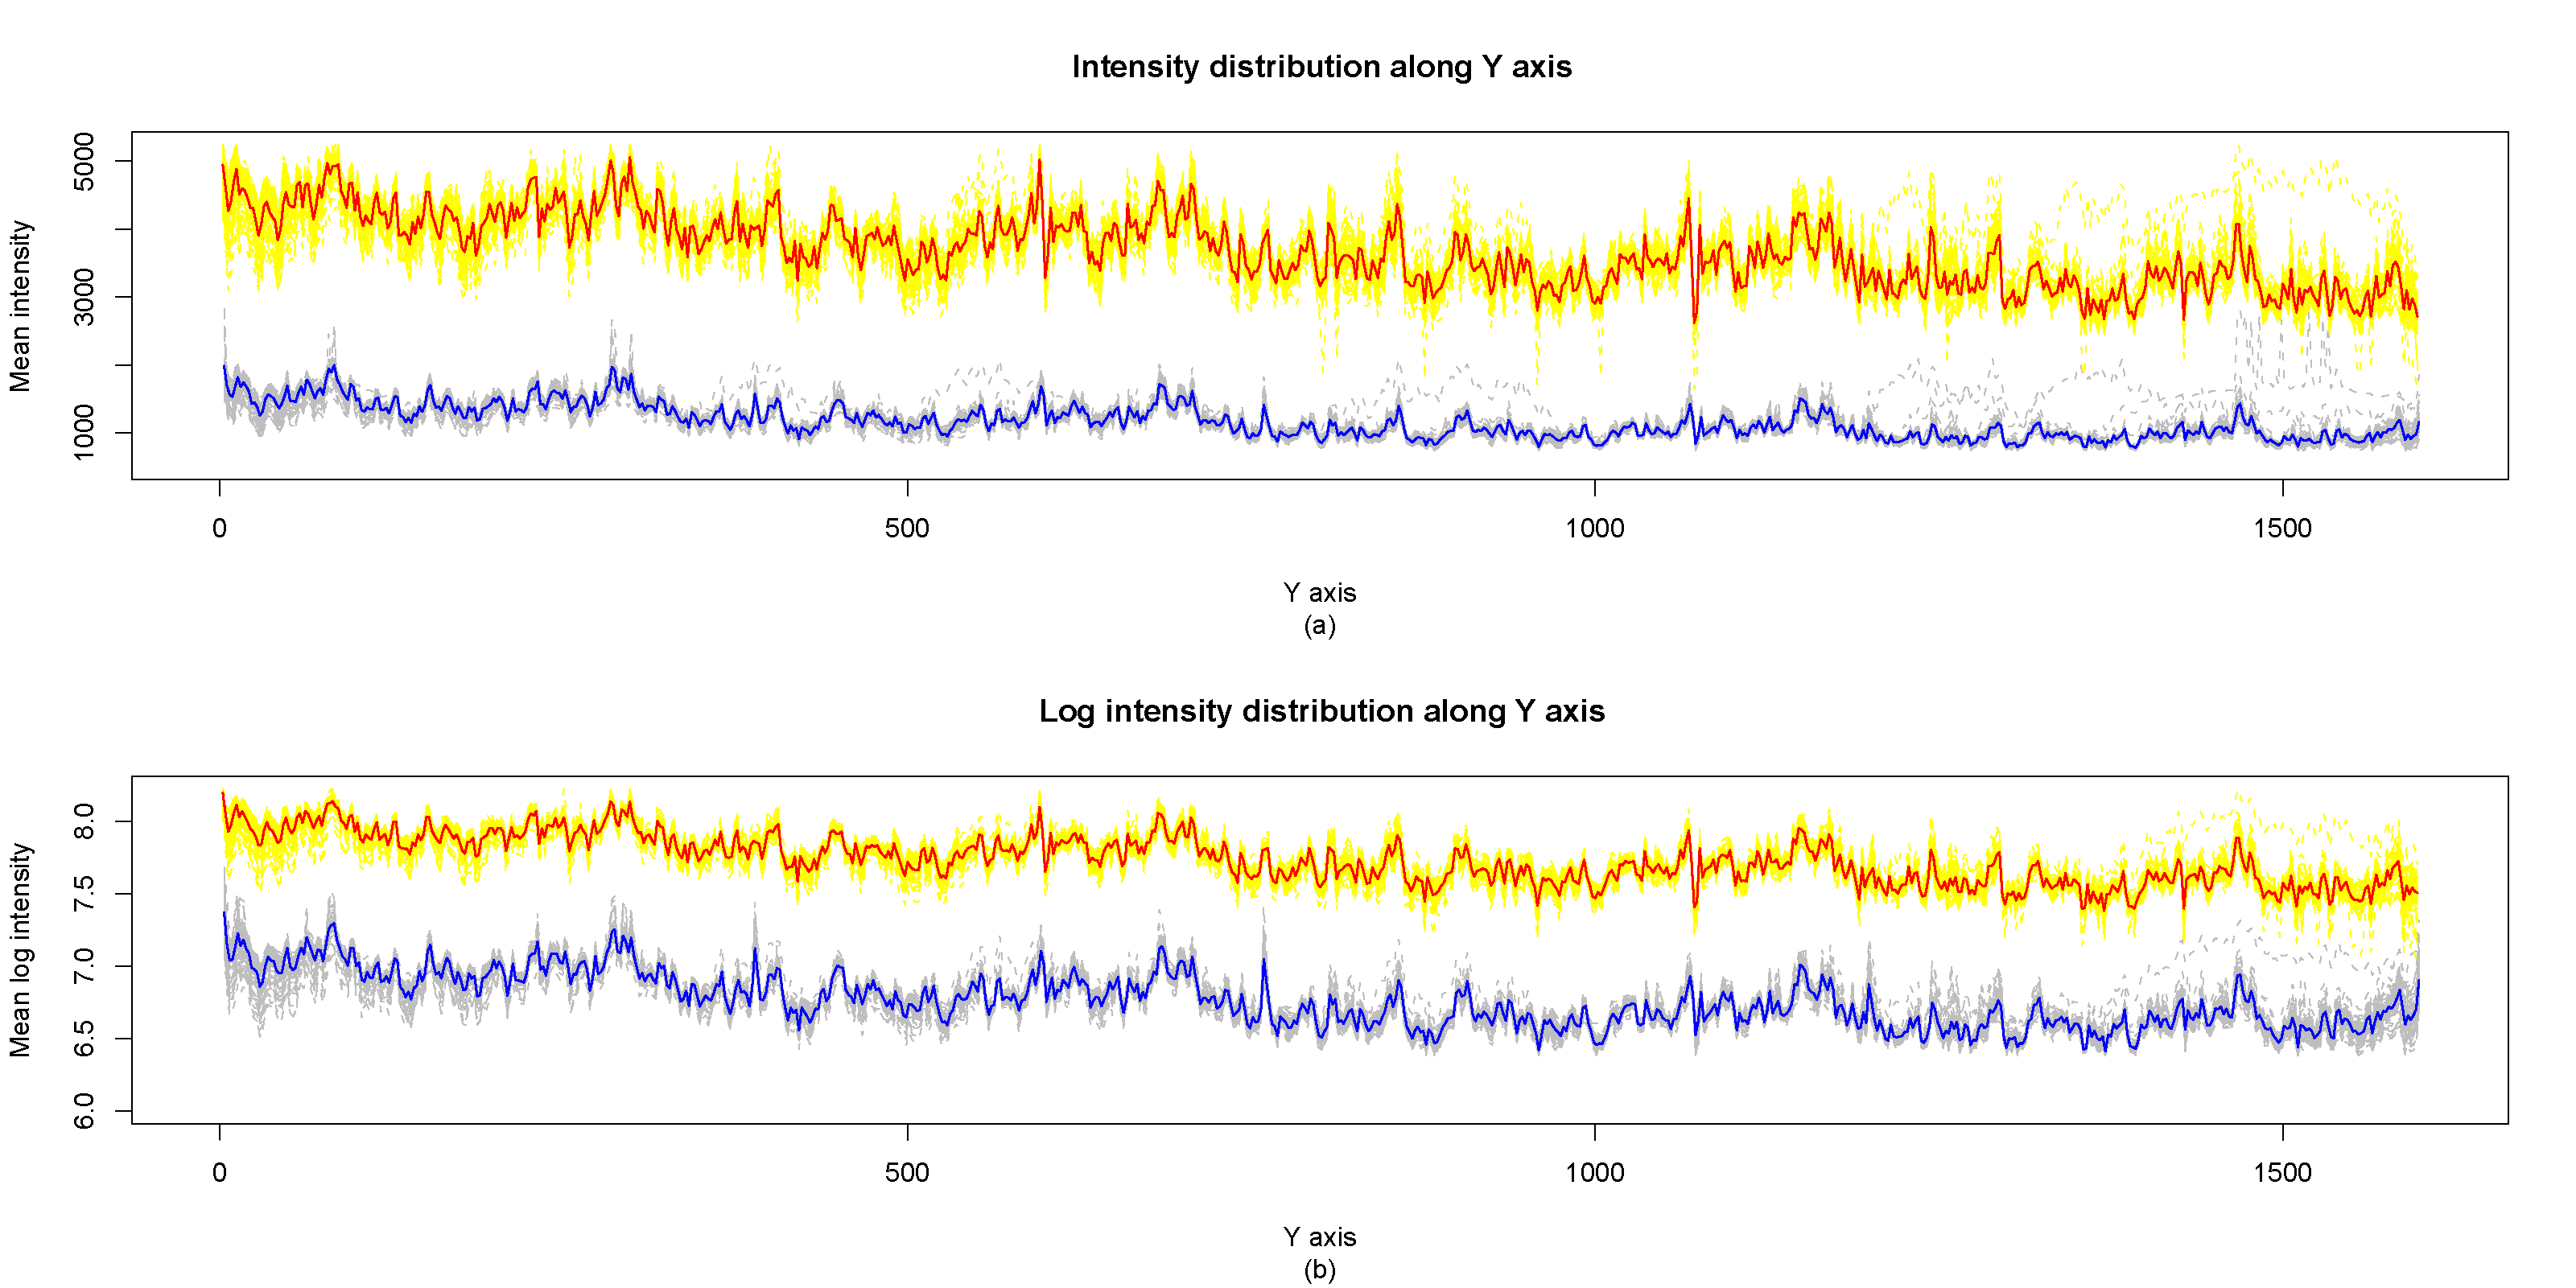
\includegraphics[width = \textwidth]{./figures/2a.png}
		\caption{This is the format for referencing parts of a figure.}\label{subfig:2a}
	\end{subfigure}
	\quad
	\begin{subfigure}[b]{.4\textwidth}
		\centering
		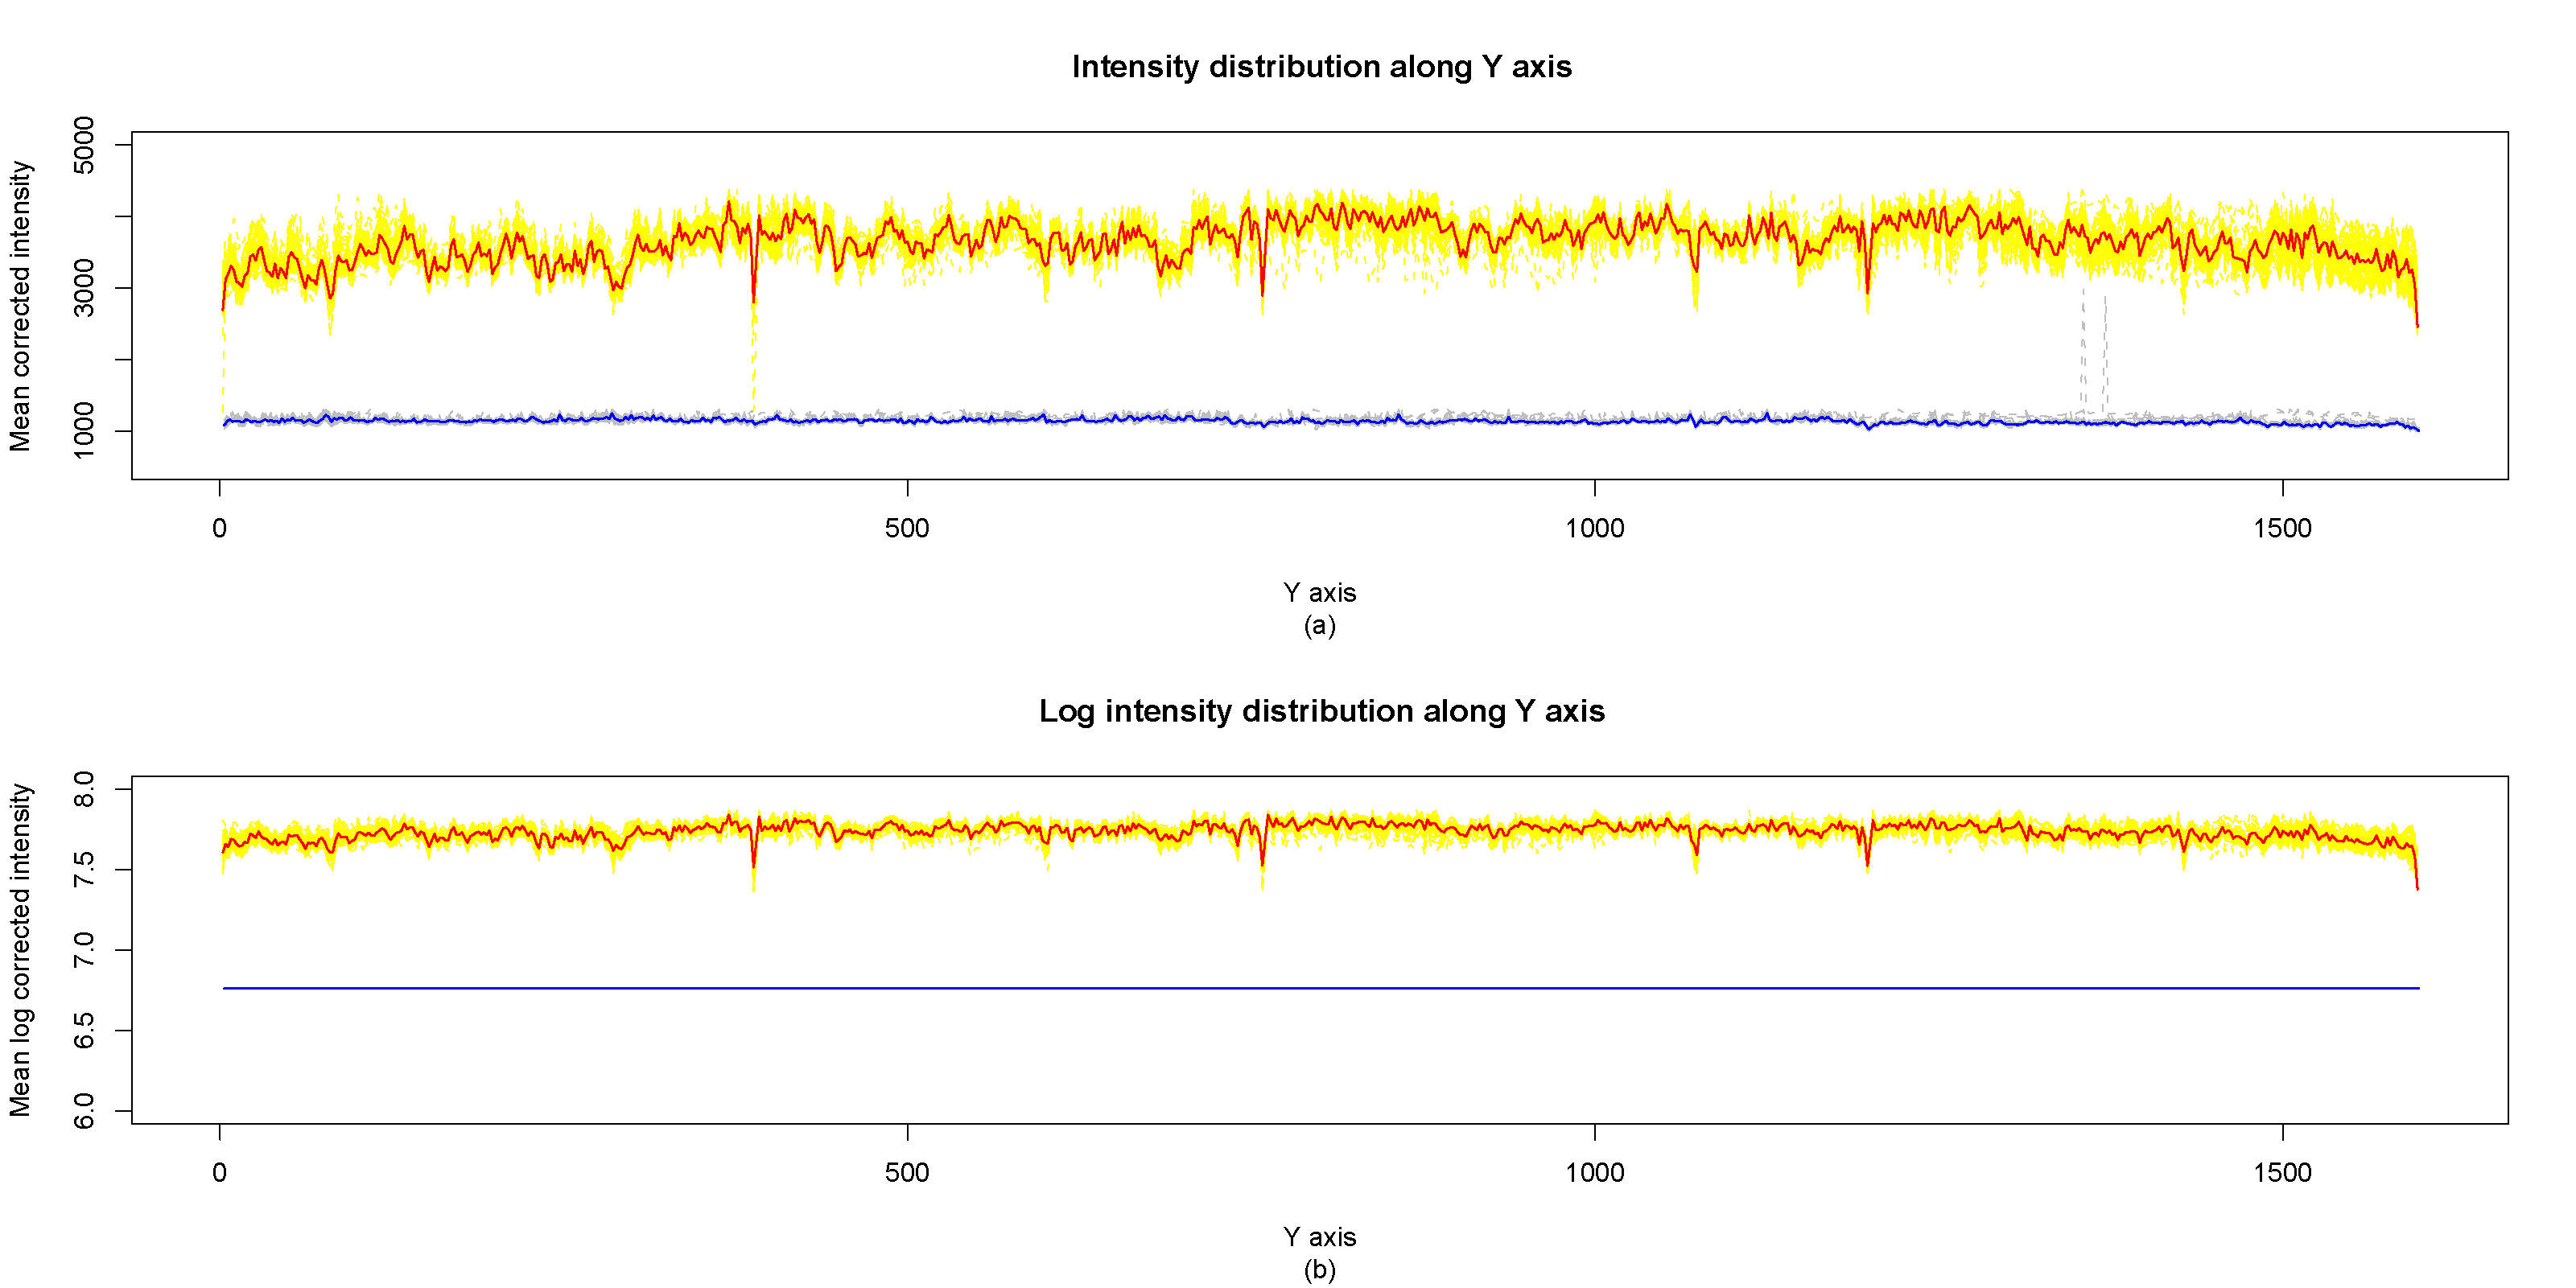
\includegraphics[width = \textwidth]{./figures/2b.png}
		\caption{This is the format for referencing parts of a figure.}\label{subfig:2b}
	\end{subfigure}
	\caption{Example of a TWO-COLUMN figure caption: (a) this is the format for referencing parts of a figure.}
	\label{fig:subfig}
\end{figure*}

\section*{Citation Specification}
List and number all bibliographical references in 9-point Times, single-spaced, at the end of your paper. When referenced in the text, enclose the citation number in square brackets, for example \cite{b1}. Where appropriate, include the name(s) of editors of referenced books. The template will number citations consecutively within brackets \cite{b1}. The sentence punctuation follows the bracket \cite{b2}. Refer simply to the reference number, as in \cite{b3}—do not use "Ref. \cite{b3}" or "reference \cite{b3}" except at the beginning of a sentence: "Reference \cite{b3} was the first . . ."

Number footnotes separately in superscripts. Place the actual footnote at the bottom of the column in which it was cited. Do not put footnotes in the reference list. Use letters for table footnotes.

Unless there are six authors or more give all authors’ names; do not use "et al.". Papers that have not been published, even if they have been submitted for publication, should be cited as "unpublished" \cite{b4}. Papers that have been accepted for publication should be cited as "in press" \cite{b5}. Capitalize only the first word in a paper title, except for proper nouns and element symbols.

For papers published in translation journals, please give the English citation first, followed by the original foreign-language citation \cite{b6}.

\begin{thebibliography}{00}
	\bibitem{b1} G. Eason, B. Noble, and I. N. Sneddon, “On certain integrals of Lipschitz-Hankel type involving products of Bessel functions,” Phil. Trans. Roy. Soc. London, vol. A247, pp. 529–551, April 1955. 
	\bibitem{b2} J. Clerk Maxwell, A Treatise on Electricity and Magnetism, 3rd ed., vol. 2. Oxford: Clarendon, 1892, pp.68–73.
	\bibitem{b3} I. S. Jacobs and C. P. Bean, “Fine particles, thin films and exchange anisotropy,” in Magnetism, vol. III, G. T. Rado and H. Suhl, Eds. New York: Academic, 1963, pp. 271–350.
	\bibitem{b4} K. Elissa, “Title of paper if known,” unpublished.
	\bibitem{b5} minutes
	\bibitem{b6} R. Nicole, “Title of paper with only first word capitalized,” J. Name Stand. Abbrev., in press.
	\bibitem{b7} Y. Yorozu, M. Hirano, K. Oka, and Y. Tagawa, “Electron spectroscopy studies on magneto-optical media and plastic substrate interface,” ASME Transl. J. Magn. Japan, vol. 2, pp. 740–741, August 1987 [Digests 9th Annual Conf. Magnetics Japan, p. 301, 1982].
	\bibitem{b8} M. Young, The Technical Writer’s Handbook. Mill Valley, CA: University Science, 1989.
	\bibitem{b9} Electronic Publication: Digital Object Identifiers (DOIs):
	Article in a journal:
	\bibitem{b10} D. Kornack and P. Rakic, “Cell Proliferation without Neurogenesis in Adult Primate Neocortex,” Science, vol. 294, Dec. 2001, pp. 2127-2130, doi:10.1126/science.1065467.
	\bibitem{b11} H. Goto, Y. Hasegawa, and M. Tanaka, “Efficient Scheduling Focusing on the Duality of MPL Representatives,” Proc. ASME Symp. Computational Intelligence in Scheduling (SCIS 07), ASME Press, Dec. 2007, pp. 57-64, doi:10.1109/SCIS.2007.357670.
\end{thebibliography}

\begin{table*}[h]
	\centering  \def\arraystretch{1.5}   %表格间距
	\begin{tabular}{|c|c|c|c|c|}
		\multicolumn{5}{l}{This form helps us to understand your paper better, {\color{red} the form itself will not be published.}} \\
		\hline 
		\bfseries Your Name & \bfseries Title$^{\mathrm{*}}$ & \bfseries Affiliation &\bfseries Research Field & \bfseries Personal Webpage \\ 
		\hline 
		&  &  &  &  \\ 
		\hline 
		&  &  &  &  \\ 
		\hline 
		&  &  &  &  \\ 
		\hline 
		&  &  &  &  \\ 
		\hline 
		\multicolumn{5}{l}{$^{\mathrm{*}}$Title can be chosen from: master student, Phd candidate, assistant professor, lecture, senior lecture, associate professor, full professor}
	\end{tabular} 
\end{table*}

\end{document}
